\documentclass[12pt,a4paper]{article}

% ---------- packages ----------
\usepackage[margin=1in]{geometry}
\usepackage{setspace}
\usepackage[switch]{lineno}
\usepackage{graphicx}
\usepackage{booktabs}
\usepackage{array}
\usepackage[super,comma,sort&compress]{natbib}
\usepackage[labelfont=bf,font=small,justification=justified,singlelinecheck=false]{caption}
\usepackage{authblk}
\usepackage{amsmath}
\usepackage{textcomp}
\usepackage{microtype}
\usepackage[hidelinks,breaklinks]{hyperref}

\graphicspath{{../results/pub_figs/main/}{../results/pub_figs/supp/}}
\renewcommand{\figurename}{Figure}
\bibliographystyle{unsrtnat}
\setlength{\bibsep}{2pt plus 0.3ex}
\renewcommand\Affilfont{\small\normalfont}
\setcounter{secnumdepth}{0}

% ---------- title ----------
\title{\bfseries A cross-cohort single-cell and spatial atlas of human H3K27M-altered diffuse midline glioma}
\author[1]{[Author One]}
\author[1,2]{[Author Two]}
\author[1,*]{[Senior Author]}
\affil[1]{[Department, Institution, City, Country]}
\affil[2]{[Second affiliation]}
\affil[*]{Correspondence: [email]}
\date{}

\begin{document}
\sloppy
\maketitle
\thispagestyle{empty}

\noindent\textbf{Keywords:} diffuse midline glioma; H3K27M; single-cell RNA sequencing; single-nucleus RNA
sequencing; spatial transcriptomics; data integration; reference atlas

\vspace{1em}
\noindent\textbf{Manuscript type:} Resource. \quad \textbf{Main figures:} 5. \quad \textbf{Tables:} 4. \quad
\textbf{Supplementary items:} 7 figures, 1 table.

\vspace{1.2em}
\noindent\textbf{Highlights}
\begin{itemize}\setlength\itemsep{0.1em}
  \item A harmonized reference of 311,618 cells from 57 human H3K27M DMG samples and 52 patients
  \item Only 2 of 15 malignant expression programmes recur across studies and both assay types
  \item Every lineage-identity programme is nuclei-restricted; dissociation stress is cell-restricted
  \item Mesenchymal tumour co-localises with myeloid cells; the OPC-oligodendroglial pairing does not
\end{itemize}

\vspace{0.6em}
\noindent\textbf{In brief}

\noindent [Authors] integrate six published single-cell and single-nucleus datasets of H3K27M diffuse midline
glioma into a harmonized 52-patient reference, then use it to show that most malignant expression programmes are
assay-dependent rather than reproducible features of the disease. The atlas serves as a reference for mapping new
DMG data.

\newpage
\doublespacing
\linenumbers

\section{Summary}

H3K27M-altered diffuse midline glioma (DMG) is uniformly lethal, and the single-cell literature describing it is
fragmented across small cohorts that differ in dissociation protocol, assay and anatomical site. We integrated six
published human DMG datasets into a harmonized reference of 311,618 cells and nuclei from 57 samples and 52
patients, with lineage labels that transfer to entirely held-out patients at 0.975 accuracy and malignant calls
that agree with the original annotations in a median 89.8\% of cells per sample. Applying a replication rule
stated before the analysis, only 2 of 15 malignant expression programmes recur across three studies and both assay
types, because every lineage-identity programme in these data is nuclei-restricted. In 21 Visium sections from 12
patients, a pre-stated mesenchymal--myeloid association holds while a pre-stated oligodendroglial one does not.
The atlas is released as a reference for mapping new DMG data.

\section{Introduction}

Diffuse midline glioma with an H3 K27 alteration is a distinct WHO grade 4 entity of the pons, thalamus and spinal
cord, and remains incurable: median survival is under a year and no systemic therapy has altered that
\citep{louis2021who,mackay2017integrated,hoffman2018clinical}. The defining lesion, a lysine-to-methionine
substitution at position 27 of histone H3, was identified in paediatric glioblastoma and diffuse intrinsic pontine
glioma \citep{schwartzentruber2012driver,wu2012somatic} and acts by inhibiting PRC2, producing global loss of
H3K27me3 with focal retention and widespread H3K27 acetylation
\citep{lewis2013inhibition,bender2013reduced,harutyunyan2019hkm,krug2019pervasive}. The resulting transcriptional
dependencies \citep{nagaraja2017transcriptional}, the capacity of these tumours to integrate electrically into neural
circuits \citep{venkatesh2019electrical} and their subclonal functional diversity \citep{vinci2018functional} have all
been mapped, yet neither targeted epigenetic therapy \citep{arrillagaromany2024onc} nor cellular immunotherapy
\citep{majzner2022gdcar} has produced durable remission.

Single-cell studies established that DMG is dominated by an oligodendrocyte-precursor-like (OPC-like) compartment with
smaller astrocyte-like (AC-like) and oligodendrocyte-like (OC-like) fractions, a picture first drawn from 3,321 cells
across six patients \citep{filbin2018developmental} and subsequently refined by developmental anchoring in canonical
and non-canonical H3 variants \citep{jessa2022km,jessa2019stalled} and by age-stratified analysis of tumour cell states
\citep{liu2022landscape}. The conceptual framework --- a hierarchy of cycling progenitor-like cells differentiating
into more mature states --- parallels adult glioblastoma \citep{patel2014singlecell,neftel2019integrative}. The
microenvironment has been characterised as non-inflammatory and microglia-dominated
\citep{lin2018noninflammatory,ross2024microglia}, with candidate immune checkpoints emerging from recent cohorts
\citep{collot2026igsfvista}, and spatial studies have begun to place these states in tissue
\citep{ren2023spatial,huchede2024bmp}.

Three problems limit how far that literature can be pushed. First, every individual DMG cohort is small; few public
deposits contain more than ten patients, so sample-level inference is underpowered and patient-level inference rarer
still. Second, the deposits differ in ways confounded with the biology of interest: pontine tumours are sampled at
autopsy as frozen nuclei \citep{okada2026singlenucleus} while thalamic tumours are more often resected and dissociated
as whole cells \citep{desisto2024tumor}, so assay, site and clinical context cannot be separated within any one study.
Third, published cell states are typically derived per study, so it is unclear which are reproducible features of the
disease and which are properties of a protocol --- a concern made concrete by pan-cancer work showing that recurrent
expression programmes can be recovered consistently only when tested across many tumours
\citep{gavish2023hallmarks}.

An integrated reference addresses the first problem and makes the second and third testable. Variational autoencoders
trained with batch covariates \citep{lopez2018deep} and their semi-supervised extension for label transfer
\citep{xu2021probabilistic} are standard for atlas assembly, with transfer learning allowing new datasets to be placed
in an existing reference \citep{lotfollahi2021mapping} and established metrics for judging whether batch effect was
removed at the cost of biology \citep{luecken2021benchmarking}. We applied this machinery to every human H3K27M DMG
single-cell deposit we could obtain and treated the limitations as first-class results: we pre-registered a replication
rule for expression programmes, kept patients rather than cells as the unit of inference wherever a claim concerns
tumours, and submitted the finished analysis to an adversarial audit followed by independent verification of every
correction.

\section{Results}

\subsection{A 311,618-cell integrated reference from six human DMG cohorts}

We screened the public single-cell landscape for human H3K27M DMG and retained six studies as a reference cohort, with
five further cohorts reserved for projection-only validation (Supplementary Table~1). Quality control was applied per
assay class, and of 420,381 cells in atlas-eligible samples 356,406 passed (84.8\%); the reference was then restricted
to samples with recoverable unique molecular identifier counts, giving \textbf{311,618 cells and nuclei from 57 samples
and 52 patients} measured over the 18,882 genes detected in every contributing study (Table~\ref{tab:cohort},
Figure~\ref{fig:atlas}a). One autopsy series dominates: Okada 2026 contributes 156,936 nuclei from 22 patients
(50.4\%) \citep{okada2026singlenucleus}, followed by Jessa 2022 single-cell and single-nucleus data (83,076 cells, 17
patients), the same study's multiome RNA (46,288 nuclei, 10 patients) \citep{jessa2022km}, Collot 2026 (17,562 nuclei,
4 patients) \citep{collot2026igsfvista}, Zang 2024 (6,546 cells, 1 patient) \citep{zang2024singlecell} and DeSisto
2024 (1,210 cells, 2 patients) \citep{desisto2024tumor}. By assay the reference is 229,043 single-nucleus, 46,288
multiome RNA and 36,287 whole-cell profiles --- 88.4\% nuclei --- and by site 42 pontine and 15 thalamic samples. The
H3 variant is reported for only 32 of 57 samples (8 H3.1, 1 H3.2, 23 H3.3); the remaining 25 are DMG by deposited
diagnosis.

Integration with scVI \citep{lopez2018deep} (three seeds, 3,000 highly variable genes selected per sample
\citep{stuart2019comprehensive}, sample as batch, study, assay and mitochondrial fraction as covariates) was compared
against Harmony \citep{korsunsky2019fast} and uncorrected principal components using scIB-style metrics
\citep{luecken2021benchmarking}. The pre-stated selection score --- $0.4 \times$ batch mixing $+\ 0.6 \times$
biological conservation --- chose scVI seed 1 at \textbf{0.739} (batch 0.537, biology 0.874) over Harmony at 0.581
(0.736, 0.478) and principal components at 0.126 (0.127, 0.125) (Figure~\ref{fig:atlas}e, Supplementary Figure~2).
Harmony mixes batches more aggressively but at a cost in biological structure that the weighting rejects. In the chosen
embedding, malignant cells form a single large territory while myeloid, oligodendrocyte, astrocyte, neuronal, vascular
and T/NK compartments separate cleanly, and samples from all six studies and all three assays intermingle within each
compartment (Figure~\ref{fig:atlas}b--d).

\begin{figure}[htbp]
\centering
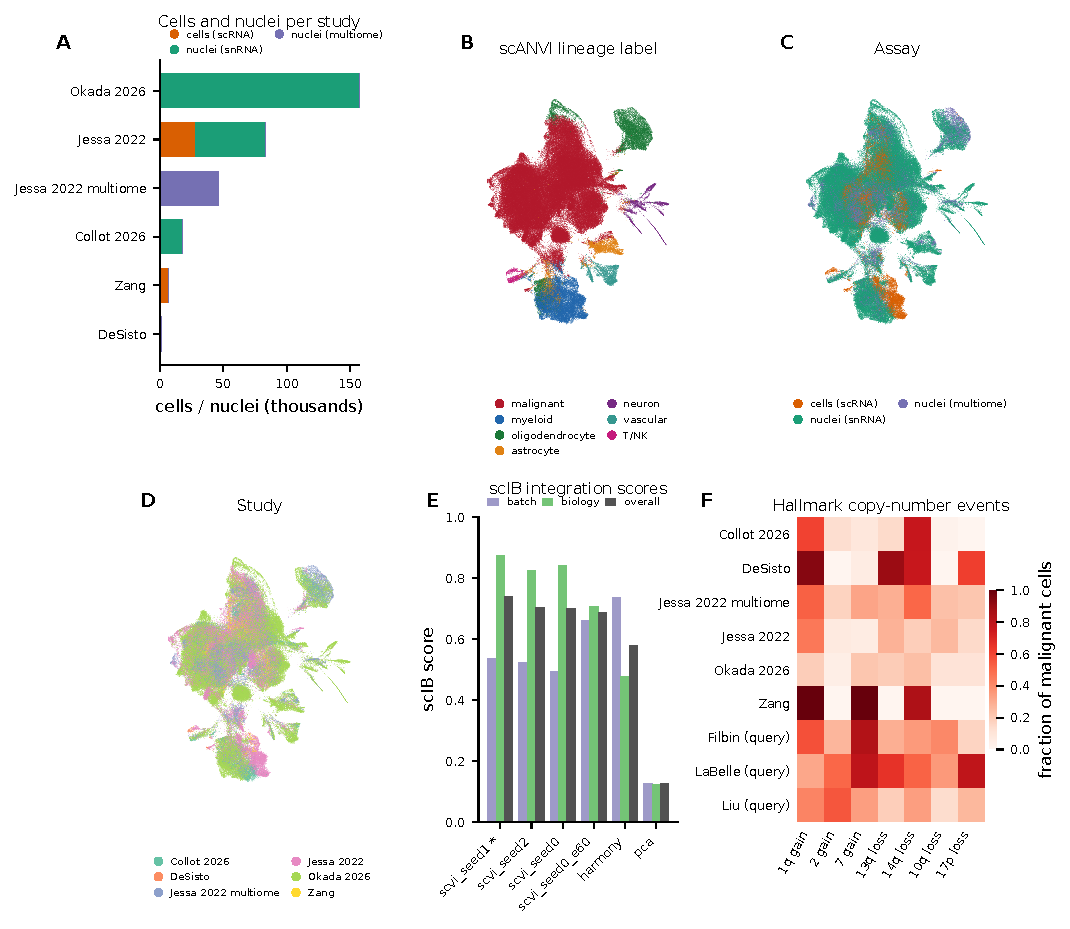
\includegraphics[width=\textwidth]{fig1_atlas.pdf}
\caption{\textbf{An integrated reference of human H3K27M diffuse midline glioma.}
\textbf{a}, Cells and nuclei per contributing study, coloured by assay.
\textbf{b--d}, UMAP of the scANVI latent space (computed on ``X\_scanvi'' with 30 neighbours; 311,618 cells, 57 samples,
52 patients), coloured by harmonised
lineage label (b), assay (c) and study (d).
\textbf{e}, scIB-style integration metrics for three scVI seeds, a 60-epoch scVI variant, Harmony and uncorrected
principal components, separated into batch-mixing, biological-conservation and overall scores; the asterisk marks the
model selected by the pre-stated 0.4/0.6 score.
\textbf{f}, Fraction of copy-number-malignant cells carrying each recurrent arm-level event, by study, including the
two projection-only cohorts.}
\label{fig:atlas}
\end{figure}

\begin{table}[htbp]
\centering\footnotesize
\caption{\textbf{Reference cohort.} Samples, patients and cells per contributing study after quality control, with
assay, anatomical site and reported H3 variant (sample counts), and the fraction of cells called malignant by the
consensus rule. Counts are cells for whole-cell and nuclei for single-nucleus and multiome assays.}
\label{tab:cohort}
\resizebox{\textwidth}{!}{%
\begin{tabular}{lrrrlllr}
\toprule
Study & Samples & Patients & Cells & Assay (cells) & Site (samples) & H3 variant (samples) & Malignant \\
\midrule
Okada 2026 & 22 & 22 & 156,936 & snRNA:156936 & thalamus:6;pons:16 & unknown:22 & 0.516 \\
Jessa 2022 (sc/snRNA) & 17 & 17 & 83,076 & snRNA:54545;scRNA:28531 & pons:13;thalamus:4 & H3.1:6;H3.2:1;H3.3:10 & 0.566 \\
Jessa 2022 (multiome) & 10 & 10 & 46,288 & multiome\_RNA:46288 & pons:9;thalamus:1 & H3.1:2;H3.3:8 & 0.595 \\
Collot 2026 & 5 & 4 & 17,562 & snRNA:17562 & pons:3;thalamus:2 & H3.3:5 & 0.570 \\
Zang 2024 & 1 & 1 & 6,546 & scRNA:6546 & pons:1 & unknown:1 & 0.710 \\
DeSisto 2024 & 2 & 2 & 1,210 & scRNA:1210 & thalamus:2 & unknown:2 & 0.631 \\
\midrule
Total & 57 & 56 & 311,618 & \multicolumn{4}{l}{18,882 genes shared by all studies} \\
\bottomrule
\end{tabular}}
\end{table}


\subsection{Malignant-cell calling agrees with published annotations in nine of ten cells}

Malignant status was assigned per cell by combining lineage-marker scoring with an expression-based copy-number profile
computed against within-sample immune and oligodendrocyte references \citep{patel2014singlecell}, smoothed over
100-gene windows and summarised both chromosome-wide and per chromosome arm (Methods). We evaluated the calls against
the original authors' annotations wherever they exist: \textbf{324,676 annotated cells across 97 samples}, with
agreement computed per sample so that large cohorts cannot dominate (Table~\ref{tab:cnv}). The median per-sample
agreement is \textbf{0.898 (IQR 0.793--0.978)}; the unweighted mean is 0.836 (95\% CI 0.790--0.877) and the
cell-weighted pooled value 0.884 (precision 0.934, recall 0.909), the gap reflecting poorer performance in small
Smart-seq2 plates and low-complexity nuclei samples (Supplementary Figure~1). Thresholds were tuned on 22 samples;
agreement on those samples (0.882) is indistinguishable from the 75 held-out ones (0.885), so the calls are not an
artefact of tuning. Calls supported by at least one recurrent arm-level event are more reliable than score-only calls
(precision 0.952 versus 0.862), and we therefore ship the event support as a confidence field rather than a filter.

Recurrent events behave as expected for the disease: chromosome 1q gain is the most frequent, followed by 14q and 13q
loss, with 17p loss confined to a minority of samples (Figure~\ref{fig:atlas}f). We explicitly dropped 4q12
(\textit{PDGFRA}/\textit{KIT}) from the hallmark set: at 100-gene resolution that band is covered by at most one
window, and what it measures is OPC-lineage expression against an immune reference rather than copy number --- the
apparent 4q12 gain frequencies in the TPM-based cohorts were lineage expression, and gene-level deviations are released
for exploratory use only. Combining marker and copy-number evidence leaves 182,924 cells (53.5\%) called malignant,
60,026 normal and 99,263 (29.0\%) ambiguous; a permissive variant that trusts event-backed copy-number calls over
discordant markers recovers a further 30,463 cells and is released as a sensitivity label.

\begin{table}[htbp]
\centering\footnotesize
\caption{\textbf{Agreement of malignant calls with published annotations.} Tier-2 comparison of the copy-number call
against each study's own annotation, for every annotated cell. Pooled values weight cells equally; the sample median
(with interquartile range) and unweighted sample mean weight samples equally.}
\label{tab:cnv}
\resizebox{\textwidth}{!}{%
\begin{tabular}{lrrrrrlr}
\toprule
Study & Cells & Samples & Agreement & Precision & Recall & Sample median (IQR) & Sample mean \\
\midrule
Jessa 2022 (sc/snRNA) & 84,194 & 17 & 0.915 & 0.982 & 0.914 & 0.898 (0.835--0.964) & 0.846 \\
Jessa 2022 (multiome) & 46,618 & 10 & 0.935 & 0.948 & 0.967 & 0.948 (0.897--0.988) & 0.930 \\
Collot 2026 & 17,750 & 5 & 0.907 & 0.896 & 0.975 & 0.960 (0.919--0.964) & 0.929 \\
Okada 2026 & 161,043 & 22 & 0.850 & 0.906 & 0.890 & 0.868 (0.763--0.895) & 0.800 \\
Liu 2022 (query) & 8,705 & 42 & 0.799 & 0.975 & 0.782 & 0.945 (0.770--0.990) & 0.813 \\
LaBelle (query) & 6,366 & 1 & 1.000 & nan & nan & 1.000 (1.000--1.000) & 1.000 \\
\textbf{\textbf{All}} & \textbf{324,676} & \textbf{97} & \textbf{0.884} & \textbf{0.934} & \textbf{0.909} & \textbf{0.898 (0.793--0.978)} & \textbf{0.836} \\
\bottomrule
\end{tabular}}
\end{table}


\subsection{Lineage labels transfer to held-out patients and to five external cohorts}

A scANVI classifier \citep{xu2021probabilistic} trained on all labelled reference cells, with the validation split made
by \textbf{patient} rather than by cell, reaches 0.993 training and \textbf{0.975 held-out-patient accuracy} (0.917
balanced accuracy) over 23,827 labelled cells from five patients never seen in training. Per-class recall is 0.999
malignant, 0.969 neuron, 0.950 myeloid, 0.917 oligodendrocyte, 0.896 T/NK, 0.883 vascular and 0.803 astrocyte; T/NK
precision is the weakest figure at 0.561, reflecting how few lymphocytes these tumours contain (Supplementary
Figure~2).

We then projected five cohorts deliberately excluded from training, encoding each with the frozen reference encoder and
transferring labels with no fine-tuning (Figure~\ref{fig:mapping}a--b). Two are DMG cohorts deposited as transcripts
per million rather than counts --- Filbin 2018 (3,037 cells, 9 samples) \citep{filbin2018developmental} and Liu 2022
(12,438 cells, 42 plates) \citep{liu2022landscape} --- and both land predominantly in the malignant territory (median
90.3\% and 83.6\% of cells per sample); for Liu, cells the authors called malignant are recovered as malignant in
99.3\% of cases (Figure~\ref{fig:mapping}c). An immune-focused CAR-T cohort projects as roughly half malignant and half
immune, as its composition implies. The two normal-brain references provide the specificity test: Siletti 2023 adult
pons nuclei \citep{siletti2023transcriptomic} are called malignant in a median of only \textbf{1.2\%} of cells per
dissection (1.8\% pooled), with adult oligodendrocytes, astrocytes, microglia and neuronal superclusters recovered as their matching
compartments, whereas Braun 2023 first-trimester hindbrain \citep{braun2023comprehensive} projects as 91.3\% malignant per
sample (87.7\% pooled)
(Figure~\ref{fig:mapping}d).

That last number is a property of the reference, not an error: the reference contains no normal progenitor class, so
fetal radial glia, glioblasts and neuroblasts have nowhere else to go. Their nearest neighbours are informative
nonetheless --- malignant cells sit closest to fetal glioblast (54.7\%) and oligodendroglial (32.4\%) classes, a
28.5-fold enrichment for the oligodendroglial class over its frequency in the fetal reference --- but the placement is
made at a median 15-nearest-neighbour distance of 3.28 in latent space versus 1.57 within the reference, so this is a
nearest-neighbour statement in an off-manifold region and not cell-of-origin evidence (Supplementary Figure~3). We
release the per-cell neighbour distance and uncertainty percentile so that downstream use can be filtered accordingly.

\begin{figure}[htbp]
\centering
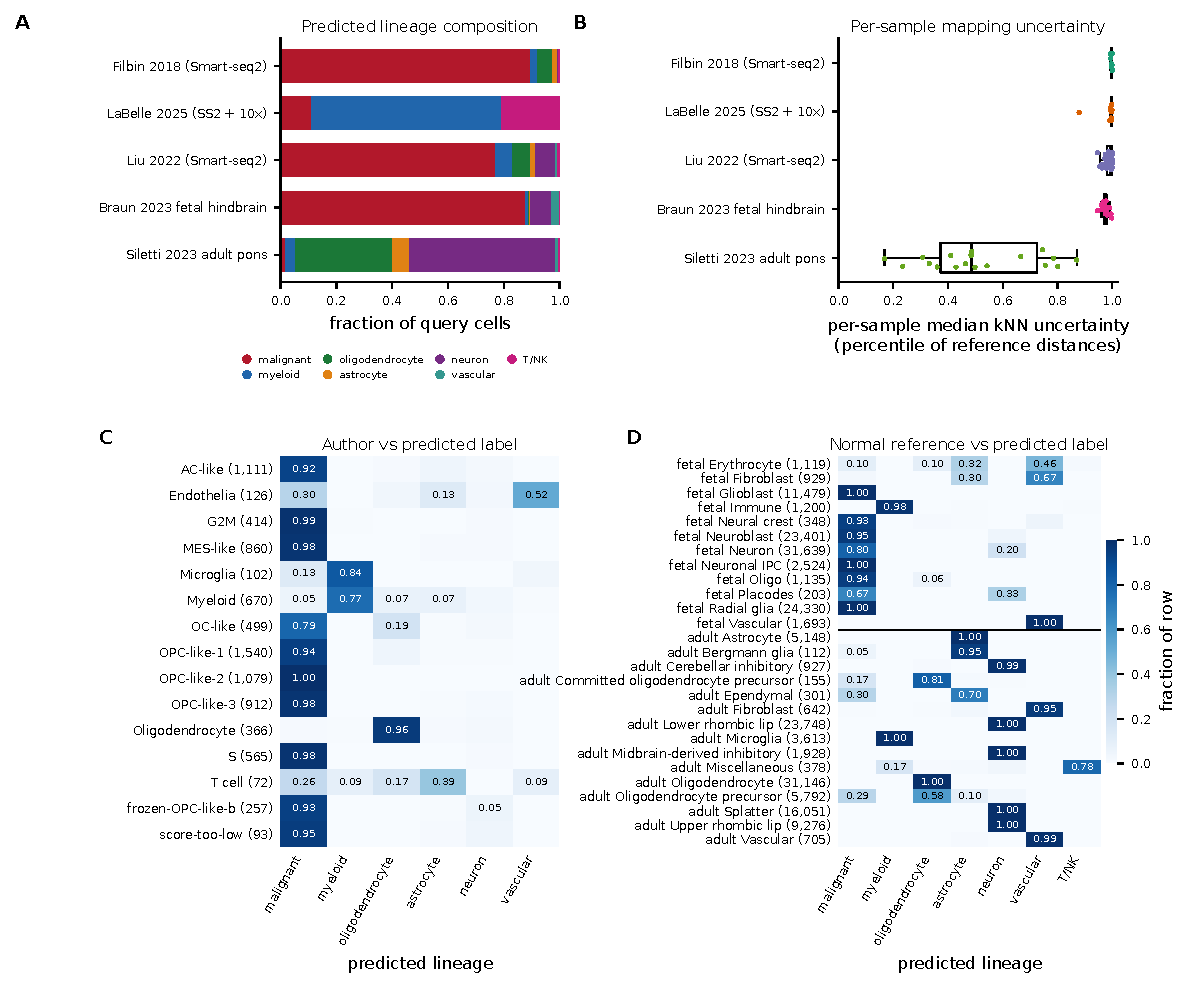
\includegraphics[width=\textwidth]{fig2_mapping.pdf}
\caption{\textbf{Zero-shot projection of five external cohorts.}
\textbf{a}, Predicted lineage composition of each query cohort.
\textbf{b}, Per-sample median neighbour-based uncertainty, expressed as a percentile of the reference's own
15-nearest-neighbour distance distribution.
\textbf{c}, Author-annotated state against predicted lineage for Liu 2022 (row-normalised).
\textbf{d}, Fetal (Braun 2023) and adult (Siletti 2023) reference classes against predicted lineage; the horizontal
rule separates the two references.}
\label{fig:mapping}
\end{figure}

\subsection{Only two of fifteen expression metaprograms replicate across studies and assays}

We derived expression programmes per sample by consensus non-negative matrix factorisation
\citep{kotliar2019identifying} on 167,012 malignant cells from 50 samples, then clustered the resulting programmes into
metaprograms. At the primary dendrogram cut, 15 metaprograms absorb 161 programmes (Table~\ref{tab:mp},
Figure~\ref{fig:mp}a, Supplementary Figure~4). Twelve carry a recognisable lineage identity --- four AC-like, two
OPC-like, one OC-like, one MES-like, two cycling, one hypoxia and one ciliated programme --- and three are technical:
ribosomal (MP2), mitochondrial (MP12) and an immediate-early-gene dissociation-stress programme (MP13).

Before deriving them we fixed a replication rule: a metaprogram counts as replicated only if it recurs in at least
three studies \textbf{and} in both whole cells and nuclei. Under that rule \textbf{2 of 15 replicate} --- cycling (MP1,
34 samples) and hypoxia (MP4, 15 samples) --- and the count is stable across dendrogram cuts from 0.84 to 0.90, rising
to 3 only at 0.91 and 5 at 0.92 (Supplementary Figure~4c). The explanation is structural rather than statistical:
\textbf{every lineage-identity programme in this cohort is nuclei-only}, and the single programme found only in whole
cells is the dissociation-stress programme. Masking the 5,921 genes that differ significantly between whole cells and
nuclei in the two paired multiome samples (plus 92 mitochondrial and ribosomal genes) and repeating the derivation
recovers 12 metaprograms with 3 replicated, against a median of 2.5 metaprograms and 1 replicated over ten
size-matched random gene masks, so the assay dependence is specific to genes that differ between cells and nuclei
rather than a generic effect of removing genes (Figure~\ref{fig:mp}b, Supplementary Figure~5).

Metaprogram families assigned per cell by within-sample standardised scores are distributed similarly in cells and
nuclei (within 0.03 per family), which is the correct comparison; the naive between-assay comparison is determined by
assay and is not interpretable (Figure~\ref{fig:mp}c--d).

\begin{figure}[htbp]
\centering
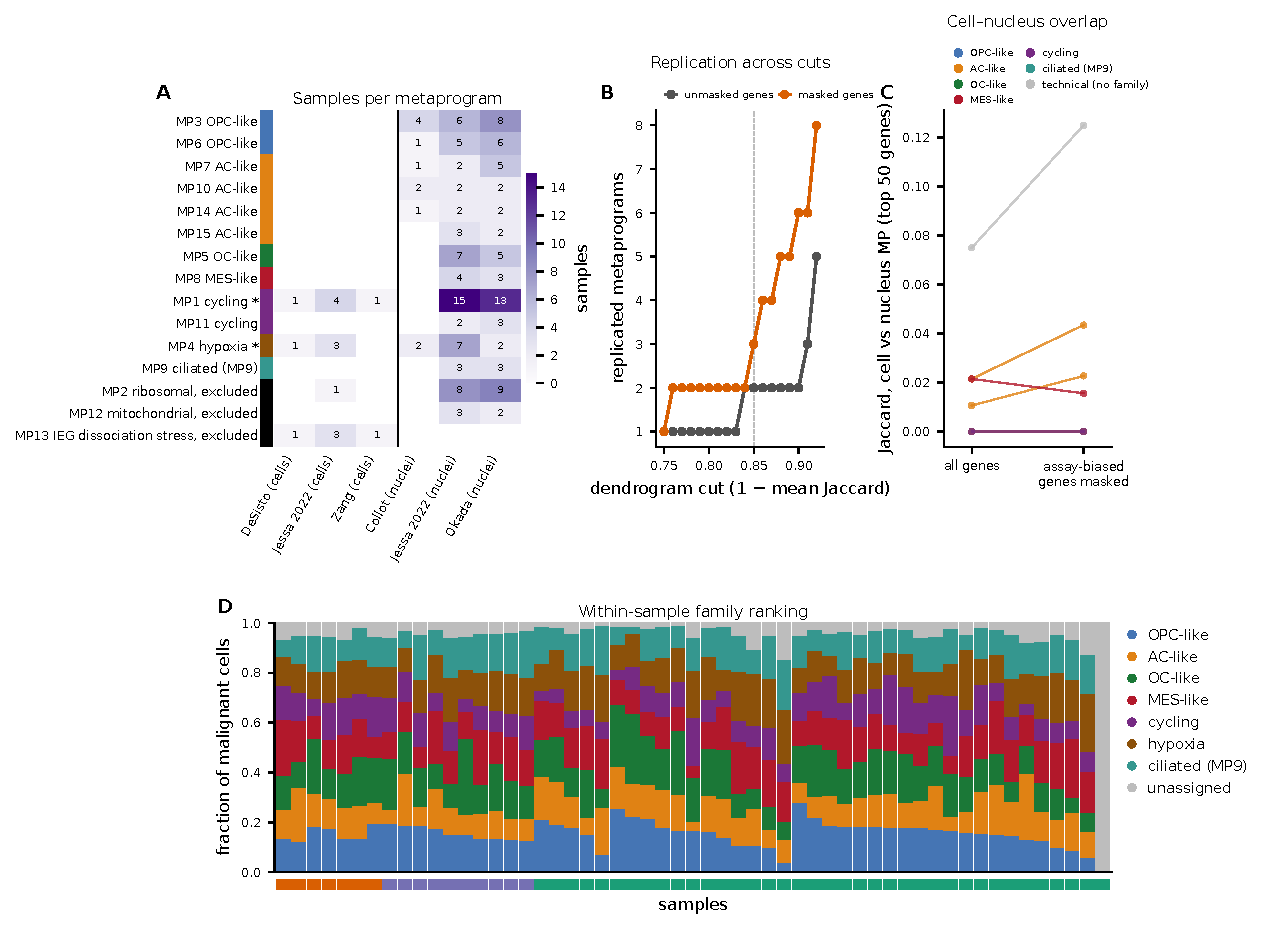
\includegraphics[width=\textwidth]{fig3_metaprograms.pdf}
\caption{\textbf{Metaprograms and their assay dependence.}
\textbf{a}, Metaprogram by study-and-assay occurrence matrix; replicated metaprograms are marked and technical
programmes are labelled by the class they capture.
\textbf{b}, Number of replicated metaprograms as a function of dendrogram cut, with and without masking the 6,013
assay-biased genes; the dashed line marks the primary cut.
\textbf{c}, Jaccard similarity between matched cell-derived and nucleus-derived metaprograms, by family, before and
after assay masking.
\textbf{d}, Per-sample metaprogram-family composition of malignant cells, ordered by study.}
\label{fig:mp}
\end{figure}

\begin{table}[htbp]
\centering\footnotesize
\caption{\textbf{Consensus metaprograms.} Metaprograms at the primary dendrogram cut, their assigned lineage family or
technical class, the number of samples in which a contributing programme was found, whether they satisfy the
pre-specified replication rule (at least three studies and both assay classes), and their top genes.}
\label{tab:mp}
\resizebox{\textwidth}{!}{%
\begin{tabular}{llrll}
\toprule
Metaprogram & Family & Samples & Replicated & Top genes \\
\midrule
MP1 & cycling & 34 & yes & \textit{ASPM, TOP2A, CENPF, MKI67, KIF14, TPX2} \\
MP2 & \textit{ribosomal} & 18 & no & \textit{RPL32, RPS18, RPS8, RPS27, EEF1A1, RPL8} \\
MP3 & OPC-like & 18 & no & \textit{FGF12, DSCAM, TNR, CA10, DCC, CADM2} \\
MP4 & hypoxia & 15 & yes & \textit{SLC6A6, NDRG1, AKAP12, VEGFA, HILPDA, IGFBP5} \\
MP5 & OC-like & 12 & no & \textit{TNS3, BCAS1, OPCML, GPR17, PKP4, FGF12} \\
MP6 & OPC-like & 12 & no & \textit{LHFPL3, SEZ6L, LRRC4C, KCNIP4, MMP16, SEMA5A} \\
MP7 & AC-like & 8 & no & \textit{DAAM2, NKAIN3, MGAT4C, EEPD1, DCLK1, SLC4A4} \\
MP8 & MES-like & 7 & no & \textit{CD44, NAMPT, HRH1, SAMD4A, TGFB2, TPST1} \\
MP9 & ciliated (MP9) & 6 & no & \textit{ADGB, CFAP43, DNAH9, ZBBX, MAP3K19, CFAP299} \\
MP10 & AC-like & 6 & no & \textit{SLC4A4, EEPD1, FAT3, PTPRT, ADGRV1, SLC1A3} \\
MP11 & cycling & 5 & no & \textit{BRIP1, DTL, CENPP, CENPK, RFC3, MMS22L} \\
MP12 & \textit{mitochondrial} & 5 & no & \textit{MT-CO2, MT-ND4, MT-CO3, MT-ND3, MT-CYB, MT-ATP6} \\
MP13 & \textit{IEG / dissociation stress} & 5 & no & \textit{IER2, FOS, JUNB, EGR1, JUN, FOSB} \\
MP14 & AC-like & 5 & no & \textit{DCLK1, EEPD1, SORBS1, AQP4, DAAM2, RGMA} \\
MP15 & AC-like & 5 & no & \textit{EEPD1, CD44, SPARCL1, SORBS1, SLC4A4, TNC} \\
\bottomrule
\end{tabular}}
\end{table}


\subsection{Microenvironment populations and the confounding of H3 variant with site}

Microenvironment subclustering resolves 21 populations --- homeostatic microglia, lipid-phagocytic and
hypoxic/glycolytic tumour-associated macrophages, interferon-responsive macrophages, proliferating myeloid cells,
CD4/CD8/NK lymphocyte states, five endothelial and pericyte populations, and four mature oligodendrocyte states plus a
committed OPC population (Figure~\ref{fig:tme}a, Supplementary Figure~6). The myeloid-dominated, lymphocyte-poor
composition is consistent with previous descriptions of this microenvironment
\citep{lin2018noninflammatory,ross2024microglia}. Because several of these populations are recovered almost entirely
from nuclei, we quantified assay purity directly and report it alongside the populations
(Figure~\ref{fig:tme}b).

Composition modelling across samples finds one effect that survives adjustment: neurons are more abundant in H3.1 than
H3.3 tumours ($q = 0.004$; site-adjusted $q = 0.017$; pons-only $q = 0.050$), whereas astrocyte, myeloid, vascular and
malignant-fraction differences do not survive site adjustment ($q = 0.17$--$0.27$) or restriction to pons
($q = 0.28$--$0.29$) --- all eight H3.1 samples are pontine nuclei samples, so these contrasts are confounded by design
(Figure~\ref{fig:tme}c). The strongest compositional signal in the entire analysis is technical: neurons differ between
nuclei and whole cells with a coefficient of 3.40 ($q < 10^{-9}$).

\begin{figure}[htbp]
\centering
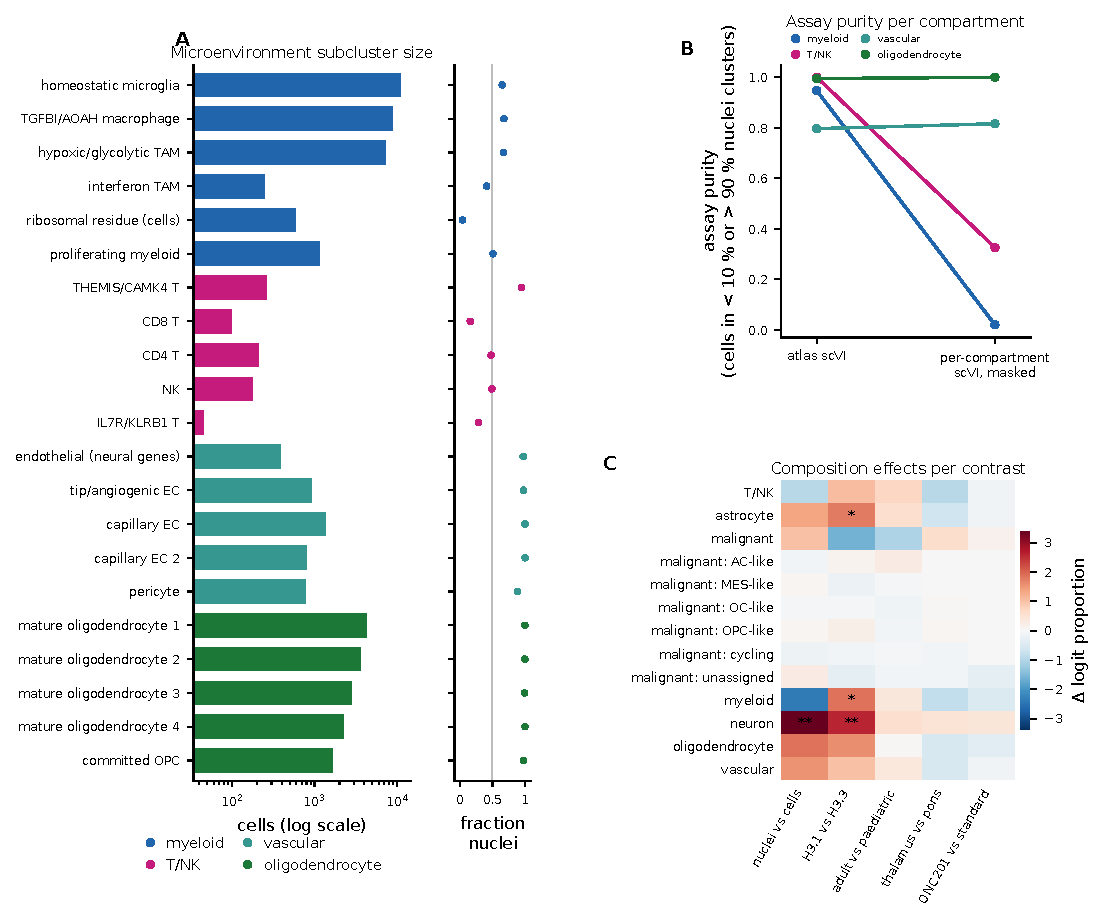
\includegraphics[width=\textwidth]{fig4_tme.pdf}
\caption{\textbf{Microenvironment populations and sample-level composition.}
\textbf{a}, Microenvironment subclusters: cell count (log scale) and the fraction of each cluster derived from nuclei.
\textbf{b}, Assay purity of microenvironment clusters in the atlas embedding versus a per-compartment model.
\textbf{c}, Composition contrasts as the change in logit proportion per cell type and malignant state; asterisks mark
Benjamini--Hochberg significance \citep{benjamini1995controlling}, and the nuclei-versus-cells column is the technical
reference contrast.}
\label{fig:tme}
\end{figure}

\subsection{Spatial co-localisation of malignant states with normal lineages}

We deconvolved 27 Visium sections from four cohorts with cell2location \citep{kleshchevnikov2022celllocation} against a
single 13-class reference built from the corrected metaprogram families (seven malignant families, six normal
lineages), and tested co-localisation on spot \textbf{proportions} with \textbf{patients} as the unit of inference: 21
DMG sections from 12 patients, Fisher-$z$ averaged within patient and pooled by random effects, with
Benjamini--Hochberg correction across 42 state-by-microenvironment pairs (Table~\ref{tab:spatial},
Figure~\ref{fig:spatial}).

Astrocyte-like tumour co-localises with normal astrocytes ($\rho = 0.393$, 95\% CI 0.234--0.531, $q = 10^{-4}$,
positive in 13 of 21 sections) and with oligodendrocytes ($\rho = 0.308$, $q = 0.005$). The ciliated programme behaves
similarly, pairing with astrocytes ($\rho = 0.369$, $q = 10^{-4}$) and showing the most consistent positive sign of any
pair with neurons ($\rho = 0.230$, $q = 10^{-4}$, positive in 16 of 21 sections). Of our two pre-stated hypotheses, the
mesenchymal one holds --- MES-like tumour co-localises with myeloid cells ($\rho = 0.238$, CI 0.071--0.392,
$q = 0.034$, 14 of 21 sections) and with vasculature ($\rho = 0.253$, $q = 0.034$) --- and the oligodendroglial one
fails: OPC-like tumour and oligodendrocytes are not associated after correction ($\rho = 0.178$, CI $-0.028$ to
$0.370$, $q = 0.210$, 10 of 21 sections). Between-patient heterogeneity is high for every pair
($I^2 = 0.952$--$0.997$), so these are small, consistent-in-sign effects rather than strong ones, and analysing
abundances instead of proportions inflates them by roughly 30\% because every class correlates with spot depth
(Supplementary Figure~7).

Ten serial sections through one whole-brainstem autopsy allow a within-tumour gradient to be described, though with one
patient it remains descriptive: within sections, tumour fraction rises with the astrocyte-like ($\rho = 0.285$, CI
0.149--0.410, positive in 9 of 10 sections) and OPC-like ($\rho = 0.213$, $q = 0.001$) share and falls with the
oligodendrocyte ($-0.298$), astrocyte ($-0.431$), vascular ($-0.235$), neuronal ($-0.239$), mesenchymal ($-0.385$) and
hypoxic ($-0.185$) shares. Finally, five DMG and five glioblastoma Visium sections deposited in a single study
\citep{ren2023spatial} permit a like-for-like comparison: DMG sections carry a higher median tumour fraction (0.528
versus 0.460) and a lower cycling share (0.112 versus 0.214), but with five sections per group neither survives
correction ($q = 0.667$ for both), and we report them as not established.

\begin{figure}[htbp]
\centering
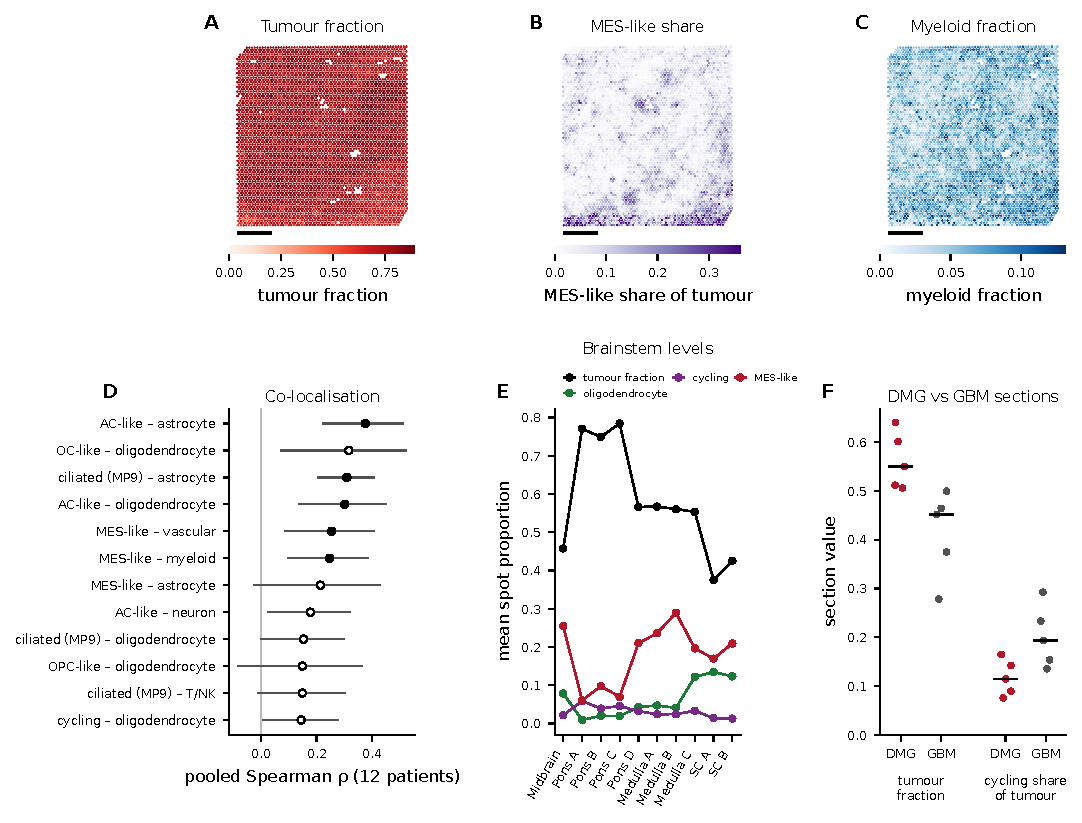
\includegraphics[width=\textwidth]{fig5_spatial.pdf}
\caption{\textbf{Spatial organisation of malignant states.}
\textbf{a--c}, One representative section (pixel coordinates, 1\,mm scale bar) showing tumour fraction, the mesenchymal
share of tumour and the myeloid fraction.
\textbf{d}, Pooled spot-level Spearman correlations between malignant states and microenvironment lineages over 12 DMG
patients and 21 sections; filled points pass Benjamini--Hochberg correction across 42 pairs.
\textbf{e}, Mean spot proportions along ten serial sections of one brainstem autopsy.
\textbf{f}, Tumour fraction and cycling share per section in five DMG and five glioblastoma sections from one study.}
\label{fig:spatial}
\end{figure}

\begin{table}[htbp]
\centering\footnotesize
\caption{\textbf{Spatial co-localisation of malignant states with microenvironment lineages.} Spot-level Spearman
correlations of cell2location proportions, Fisher-$z$ averaged within patient and pooled by random effects over 12 DMG
patients and 21 sections, Benjamini--Hochberg corrected across 42 state-by-microenvironment pairs. The ten strongest
pairs are shown; $I^2$ quantifies between-patient heterogeneity.}
\label{tab:spatial}
\resizebox{\textwidth}{!}{%
\begin{tabular}{llrlrrr}
\toprule
Malignant state & Lineage & $\rho$ & 95\% CI & $q$ & Sections $>0$ & $I^2$ \\
\midrule
AC-like & astrocyte & 0.393 & 0.234 to 0.531 & 9.38e-05 & 13/21 & 0.993 \\
ciliated (MP9) & neuron & 0.230 & 0.131 to 0.324 & 9.38e-05 & 16/21 & 0.978 \\
ciliated (MP9) & astrocyte & 0.369 & 0.216 to 0.505 & 9.38e-05 & 13/21 & 0.992 \\
AC-like & oligodendrocyte & 0.308 & 0.138 to 0.459 & 0.00512 & 11/21 & 0.993 \\
MES-like & vascular & 0.253 & 0.078 to 0.412 & 0.0339 & 13/21 & 0.993 \\
MES-like & myeloid & 0.238 & 0.071 to 0.392 & 0.0339 & 14/21 & 0.992 \\
ciliated (MP9) & oligodendrocyte & 0.235 & 0.073 to 0.385 & 0.0339 & 13/21 & 0.992 \\
OC-like & vascular & -0.214 & -0.367 to -0.051 & 0.0511 & 6/21 & 0.993 \\
ciliated (MP9) & T/NK & 0.188 & 0.044 to 0.324 & 0.0511 & 14/21 & 0.990 \\
hypoxia & T/NK & 0.082 & 0.017 to 0.147 & 0.0589 & 12/21 & 0.952 \\
\bottomrule
\end{tabular}}
\end{table}


\section{Discussion}

This resource makes three contributions. The first is the reference itself: 311,618 cells and nuclei from 52 patients
with harmonised labels, calibrated malignant calls, a frozen encoder for projection and a validated held-out-patient
classifier. For a tumour where individual cohorts contain a handful of patients, a patient-level denominator of 52 is
the difference between describing a sample and describing a disease.

The second is a set of calibrated negative results. Only two of fifteen metaprograms replicate under a rule fixed in
advance, and the reason is not noise but confounding: lineage-identity programmes appear in nuclei and the
dissociation-stress programme appears in cells, so studies profiling different material will recover different states
and agree only on cycling and hypoxia. This is a sharper version of the warning that emerges from pan-cancer programme
analysis \citep{gavish2023hallmarks}: recurrence across tumours is necessary but not sufficient when the cohorts differ
systematically in how the material was prepared. One of our two pre-stated spatial hypotheses survived patient-level
correction and the other did not. A compositional difference between H3.1 and H3.3 tumours is present for neurons and
disappears for every other cell type once site is adjusted, because H3.1 sampling is pontine sampling in these
deposits. We regard these as the most immediately useful outputs for anyone planning a DMG single-cell study: they
identify which comparisons are currently decidable from public data and which require matched material.

The third is methodological. Agreement between an expression-based copy-number call and the original authors'
annotations is not uniform --- a median of 0.898 per sample with an interquartile range spanning nearly twenty
percentage points --- and reporting it per sample rather than pooled is what exposes that. Event-backed and score-only
calls differ by nine points of precision and should not be treated alike. Zero-shot projection into a frozen reference
is accurate for tumour and adult-brain queries, and its failure mode on fetal tissue is interpretable and detectable
from the neighbour distances we release.

Several biological observations deserve follow-up in matched material. The ciliated programme is the clearest
candidate: it is the most consistently positive partner of normal neurons across sections and pairs with astrocytes as
strongly as the astrocyte-like programme does, yet it appears in no established DMG state nomenclature
\citep{filbin2018developmental,jessa2022km,liu2022landscape}. The co-localisation of mesenchymal tumour with myeloid
cells and vasculature is consistent with the hypoxia-associated mesenchymal compartment described in glioblastoma
\citep{neftel2019integrative} and with BMP-driven invasive phenotypes reported in DMG \citep{huchede2024bmp}, and the
brainstem gradient --- tumour-rich regions enriched for astrocyte-like and OPC-like programmes and depleted of normal
glia --- is what an infiltrative front is expected to look like, but a single autopsy cannot establish it. Engineered
human models that generate H3.3K27M-altered DMG \textit{de novo} in brainstem organoids \citep{bessler2026de} now offer
a route to test whether these associations are causal rather than observational.

\subsection{Limitations of the study}

One autopsy series contributes half the reference cells, and every autopsy sample in the atlas comes from it, so
autopsy versus resection is not an estimable contrast. All eight H3.1 samples are pontine nuclei samples, and the H3
variant is unreported for 25 of 57 samples. The whole-cell arm of any assay comparison rests on six samples.
Copy-number thresholds were tuned on 22 samples, and 18.9\% of malignant calls rest on the aggregate score with no
supporting arm-level event. The reference contains no normal progenitor population, so developmental queries project
into the malignant region by construction. The spatial conclusions come from 21 sections and 12 patients with high
between-patient heterogeneity, the brainstem gradient from one patient, and the DMG-versus-glioblastoma comparison from
five sections per group. Two of the eleven cohorts are deposited as transcripts per million with no recoverable counts
and are used for projection only. Metaprogram derivation was limited to nine programmes per sample in 21 of 50 samples
by cell number, so finer programmes could not be resolved.

\section{Resource availability}

\subsection{Lead contact}
Requests for further information should be directed to the lead contact, [name] ([email]).

\subsection{Materials availability}
This study did not generate new reagents or materials.

\subsection{Data and code availability}
\begin{itemize}\setlength\itemsep{0.1em}
  \item This study reanalyses published human data only. All primary accessions are listed in the key resources
        table (Table~\ref{tab:keyresources}) and Supplementary Table~1.
  \item The integrated object (\texttt{dmg\_atlas\_v1.h5ad}, CELLxGENE schema 7.x, validated with zero MUST
        failures) carries raw counts, harmonized metadata, lineage and state labels, malignant calls with
        confidence fields, and all model embeddings. \textit{Release of the merged count matrix is pending
        confirmation of redistribution terms for the post-mortem cohort, whose raw data is under controlled access
        (EGAS50000001447); if those terms preclude redistribution, the release will ship embeddings, labels and
        metadata with per-cohort pointers to the primary deposits.}
  \item All analysis code, the phase-by-phase documentation and the complete audit trail are available in the
        project repository [URL]; every figure panel records the md5 checksum of each input table.
  \item Any additional information required to reanalyse the data reported in this paper is available from the
        lead contact on request.
\end{itemize}

\section{Acknowledgments}

We thank the investigators and patients of every cohort reused here; this work exists only because those data were
deposited publicly.

\bibliography{references}

\newpage
\section{Author contributions}

[To be completed]

\section{Declaration of interests}

[To be completed]

\section{Declaration of generative AI and AI-assisted technologies in the writing process}

[To be completed: state any use of generative AI in the preparation of this manuscript, per the journal's policy.]

\section{Supplemental information}

Supplemental information includes seven supplementary figures and one supplementary table, and can be found with
this article online.

\section{STAR$\star$Methods}

\subsection{Key resources table}

\noindent See Table~\ref{tab:keyresources}.

\begin{table}[htbp]
\centering\scriptsize
\caption{\textbf{Key resources table.} Deposited data reused in this study and the software that produced the
results. Version numbers are those recorded by \texttt{scripts/28\_record\_environment.py}; the full environment
(557 conda and 167 pip entries for the local environment, plus the GPU image pins) is in \texttt{env/}.}
\label{tab:keyresources}
\setlength{\tabcolsep}{3pt}
\begin{tabular}{p{5.0cm}p{6.0cm}p{3.6cm}}
\toprule
\multicolumn{3}{l}{\textbf{Deposited data}} \\
Dataset & Identifier & Source \\
\midrule
Collot et al., DMG (snRNA) & Zenodo: 10.5281/zenodo.17922773 (scRNA.tar.gz) & Zenodo \\
DeSisto et al., paediatric HGG (scRNA) & GSE231859 & GEO \\
Jessa et al., DMG (multiome RNA) & GSE210566 & GEO \\
Jessa et al., DMG (sc/snRNA) & GSE210567 & GEO \\
Okada et al., post-mortem DMG (snRNA) & EGAS50000001447 (raw, controlled); processed matrix from the study's UCSC Cell Browser instance & EGA / UCSC Cell Browser \\
Zang et al., DMG (scRNA) & GSE245674 (GSM7846769) & GEO \\
Braun et al., first-trimester human brain & CZ CELLxGENE Discover (collection 4d8fed08-2d6d-4692-b5ea-464f1d072077) & CZ CELLxGENE \\
Filbin et al., H3K27M glioma (Smart-seq2, TPM) & GSE102130 & GEO \\
DMG immune cohort (SS2 + 10x, TPM) & GSE227983 & GEO \\
Liu et al., H3-K27M DMG (Smart-seq2, TPM) & GSE184357 & GEO \\
Siletti et al., adult human brain (pons dissections) & CZ CELLxGENE Discover (collection 283d65eb-dd53-496d-adb7-7570c7caa443) & CZ CELLxGENE \\
Whole-brainstem DIPG autopsy Visium & GSE280990 & GEO \\
Collot et al., DMG Visium & Zenodo: 10.5281/zenodo.17922773 (ST.tar.gz) & Zenodo \\
Huchede et al., DMG Visium & GSE268577 & GEO \\
Ren et al., DMG and glioblastoma Visium & GSE194329 & GEO \\
\midrule
\multicolumn{3}{l}{\textbf{Software and algorithms}} \\
Software & Reference & Identifier \\
\midrule
python v3.11.16 & Python Software Foundation & \url{https://pypi.org/project/python/} \\
numpy v2.4.6 & Harris et al. & \url{https://pypi.org/project/numpy/} \\
scipy v1.17.1 & Virtanen et al. & \url{https://pypi.org/project/scipy/} \\
pandas v2.3.3 & McKinney & \url{https://pypi.org/project/pandas/} \\
anndata v0.12.19 & Virshup et al. & \url{https://pypi.org/project/anndata/} \\
scanpy v1.11.5 & Wolf et al. & \url{https://pypi.org/project/scanpy/} \\
scikit-learn v1.7.2 & Pedregosa et al. & \url{https://pypi.org/project/scikit-learn/} \\
statsmodels v0.15.0 & Seabold and Perktold & \url{https://pypi.org/project/statsmodels/} \\
matplotlib v3.11.2 & Hunter & \url{https://pypi.org/project/matplotlib/} \\
infercnvpy v0.6.1 & Sturm et al. (inferCNV port) & \url{https://pypi.org/project/infercnvpy/} \\
leidenalg v0.12.0 & Traag et al. & \url{https://pypi.org/project/leidenalg/} \\
umap-learn v0.5.12 & McInnes et al. & \url{https://pypi.org/project/umap-learn/} \\
scvi-tools v1.4.2 & Lopez et al.; Xu et al. & \url{https://pypi.org/project/scvi-tools/} \\
torch v2.14.1 & Paszke et al. & \url{https://pypi.org/project/torch/} \\
cell2location v==0.1.5 & Kleshchevnikov et al. & \url{https://pypi.org/project/cell2location/} \\
pyro-ppl v1.9.1+ab0491a & Bingham et al. & \url{https://pypi.org/project/pyro-ppl/} \\
lifelines v0.30.3 & Davidson-Pilon & \url{https://pypi.org/project/lifelines/} \\
\bottomrule
\end{tabular}
\end{table}


\subsection{Experimental model and subject participant details}

This study reanalyses previously published human tumour and normal-brain data; no new human or animal material was
collected. Every contributing study obtained its own ethical approval and consent, as stated in the primary
publications listed in the key resources table. The reference cohort comprises 52 patients with H3K27M-altered
diffuse midline glioma (42 pontine and 15 thalamic samples); age group, anatomical site, assay and reported H3
variant per sample are given in Table~\ref{tab:cohort}. No mouse data were used.

\subsection{Method details}

\subsubsection{Cohort assembly}

Public deposits were screened by GEO E-utilities queries and a scholarly-literature search for human H3K27M DMG
single-cell and spatial data (Supplementary Table~1). Six cohorts with recoverable UMI counts form the reference (GEO
GSE210567 and GSE210566 \citep{jessa2022km}; Zenodo 10.5281/zenodo.17922773 \citep{collot2026igsfvista}; GEO GSE231859
\citep{desisto2024tumor}; GEO GSE245674, sample GSM7846769 only \citep{zang2024singlecell}; and the post-mortem series
of \citet{okada2026singlenucleus}, raw data under EGA accession EGAS50000001447 with the processed matrix obtained from
its UCSC Cell Browser instance). Five cohorts are projection-only: GEO GSE102130 \citep{filbin2018developmental} and
GSE184357 \citep{liu2022landscape}, both deposited as transcripts per million; GSE227983; and the normal-brain
references of \citet{braun2023comprehensive} (hindbrain, pons and medulla dissections, 286,973 cells) and
\citet{siletti2023transcriptomic} (six pons dissections, 204,168 nuclei), both obtained from CZ CELLxGENE Discover
\citep{abdulla2025czcellxgene}. Spatial cohorts are GSE268577 \citep{huchede2024bmp}, GSE194329 \citep{ren2023spatial}, GSE280990
and the spatial archive of Zenodo 10.5281/zenodo.17922773. One cohort (ScPCA SCPCP000021) was excluded after quality
control. All data are human; no mouse data were used.

\subsubsection{Quality control}

Thresholds were applied per assay class with distinct mitochondrial-fraction limits for whole cells and nuclei, a
minimum gene count per cell, and doublet scoring by Scrublet \citep{wolock2019scrublet} at a fixed threshold of 0.25.
Samples failing a per-sample gate were flagged and excluded from the reference but retained in the released object with
their flag. Of 420,381 cells in atlas-eligible samples, 356,406 passed; the 311,618-cell reference is the UMI-count
subset of those. All processing used Scanpy \citep{wolf2018scanpy}.

\subsubsection{Malignant-cell calling}

For each sample, cells were scored against curated lineage marker sets, and an inferCNV-style profile was computed from
log-normalised expression relative to within-sample immune and oligodendrocyte references over 100-gene windows ordered
by GENCODE v32 coordinates \citep{frankish2023gencode}, summarised both chromosome-wide and per arm. Cluster-level
calls combined an aggregate score threshold with recurrent arm-level events (1q, 2, 7 gain; 10q, 13q, 14q, 17p loss). A
three-tier consensus --- marker only, copy number only, and the agreement of both --- was evaluated against author
annotations per sample; the released \texttt{consensus\_call} requires marker and copy-number agreement, and
\texttt{consensus\_call\_eventtrust} is the permissive sensitivity variant.

\subsubsection{Integration and label transfer}

scVI \citep{lopez2018deep} was trained on 3,000 highly variable genes (Seurat v3 selection with per-sample batch
\citep{stuart2019comprehensive}) with sample as batch key, study, assay and mitochondrial fraction as covariates, 30
latent dimensions and three random seeds, on a single A10G GPU. Embeddings were compared with scIB-style metrics
\citep{luecken2021benchmarking} and selected by the pre-stated 0.4/0.6 batch/biology score; UMAP was used for
visualisation only \citep{becht2018dimensionality}. scANVI \citep{xu2021probabilistic} was initialised from the chosen
scVI model and trained on all labelled cells with the validation split stratified by patient. Query cohorts were
encoded by the frozen reference encoder without architectural surgery or fine-tuning, which the released run metadata
records as zero training epochs; labels were transferred both by the scANVI classifier and by 15-nearest-neighbour vote
in latent space \citep{lotfollahi2021mapping}, and both are released per cell with a neighbour-distance uncertainty
percentile.

\subsubsection{Metaprograms}

Per-sample consensus non-negative matrix factorisation \citep{kotliar2019identifying} was run on malignant cells from
samples with at least 200 such cells, with $k$ chosen per sample by stability and capped by cell number. Programmes
were clustered by Jaccard similarity of their top genes; the primary dendrogram cut and the pre-stated replication rule
(at least three studies and both assay classes) were fixed before inspection, and the sensitivity of both the
metaprogram count and the replication count to the cut was recorded. Per-cell family assignment used within-sample
standardised programme scores. The assay-masking control removed the 6,013 genes called assay-biased from the two
paired multiome samples (5,921 by a two-sample Welch test with consistent sign in both pairs, plus 92 mitochondrial and
ribosomal genes) and was compared against ten size-matched random masks.

\subsubsection{Spatial deconvolution and statistics}

cell2location \citep{kleshchevnikov2022celllocation} reference signatures were estimated from the 13-class
metaprogram-family reference (250 epochs), and each section was deconvolved with a wall-clock-budgeted schedule up to
20,000 epochs; realised epoch counts and full ELBO histories are released, and convergence is argued from those
histories rather than from reaching the target. Co-localisation was computed on spot proportions (with a
centred-log-ratio variant as sensitivity), Fisher-$z$ averaged within patient, pooled by DerSimonian--Laird random
effects, and corrected across 42 state-by-microenvironment pairs \citep{benjamini1995controlling}. Serial sections of
one autopsy count as one patient, as do the core and edge sections of one resection.

\subsubsection{Audit}

The completed analysis was audited by six independent adversarial reviews with no access to the reasoning that produced
it, yielding 163 findings (4 critical, 33 major). Findings were remediated in four waves and the closure of every
critical and major finding was then verified by an independent re-audit that recomputed each quantity from the released
files: 78 of 90 findings in scope verified closed, including 4 of 4 critical. The complete record --- findings, closure
claims, recomputed values and remaining open items --- is released with the atlas.

\subsection{Quantification and statistical analysis}

All analysis ran on a 14-core laptop with 24\,GB of memory except scVI/scANVI training and cell2location
deconvolution, which ran on a single A10G GPU. Software versions are recorded for both environments. Bibliographic
records were retrieved from PubMed (National Center for Biotechnology Information); DOIs for all cited works are given
in the reference list.


\newpage
\appendix
\section*{Supplementary information}
\renewcommand{\thefigure}{S\arabic{figure}}
\renewcommand{\thetable}{S\arabic{table}}
\setcounter{figure}{0}
\setcounter{table}{0}

\begin{landscape}
\footnotesize
\setlength{\tabcolsep}{4pt}\renewcommand{\arraystretch}{1.05}
\begin{longtable}{>{\raggedright\arraybackslash}p{6.2cm}>{\raggedright\arraybackslash}p{6.0cm}>{\raggedright\arraybackslash}p{3.2cm}>{\raggedright\arraybackslash}p{3.4cm}>{\raggedright\arraybackslash}p{4.6cm}}
\caption{\textbf{Public data sets screened and their use in this study.} Data sets used, with their role, followed by data
sets screened but not used, with the reason.}
\label{tab:deposits}\\
\toprule
Data set & Accession & Repository & Data type & Use in this study \\
\midrule
\endfirsthead
\toprule
Data set & Accession & Repository & Data type & Use in this study \\
\midrule
\endhead
Collot et al., DMG & 10.5281/zenodo.17922773 & Zenodo & snRNA-seq & Reference \\
DeSisto et al., paediatric HGG & GSE231859 & GEO & scRNA-seq & Reference \\
Jessa et al., DMG & GSE210566 & GEO & Multiome (RNA) & Reference \\
Jessa et al., DMG & GSE210567 & GEO & scRNA-seq, snRNA-seq & Reference \\
Okada et al., post-mortem DMG & UCSC Cell Browser (brain-dmg-multiomics); raw data EGAS50000001447 & EGA / UCSC Cell Browser & snRNA-seq & Reference \\
Zang et al., DMG & GSE245674 (GSM7846769) & GEO & scRNA-seq & Reference \\
Braun et al., first-trimester human brain & CELLxGENE collection 4d8fed08 & CZ CELLxGENE & scRNA-seq & Query (normal brain) \\
Filbin et al., H3K27M glioma & GSE102130 & GEO & Smart-seq2 (TPM) & Query (tumour) \\
LaBelle et al., DMG immune cohort & GSE227983, GSE271936 & GEO & Smart-seq2, 10x (TPM) & Query (tumour) \\
Liu et al., H3-K27M DMG & GSE184357 & GEO & Smart-seq2 (TPM) & Query (tumour) \\
Siletti et al., adult human brain & CELLxGENE collection 283d65eb & CZ CELLxGENE & snRNA-seq & Query (normal brain) \\
Whole-brainstem DIPG autopsy Visium & GSE280990 & GEO & Visium & Spatial \\
Collot et al., DMG Visium & 10.5281/zenodo.17922773 & Zenodo & Visium & Spatial \\
Huchede et al., DMG Visium & GSE268577 & GEO & Visium & Spatial \\
Ren et al., DMG and glioblastoma Visium & GSE194329 & GEO & Visium & Spatial \\
\midrule
Adult human brain Paired-Tag (Xie et al.) & GSE327101 & GEO & Paired-Tag & Not used: normal reference not required \\
PBTA / OpenPedCan v14 & -- & OpenPedCan & Bulk RNA-seq & Not used: bulk data, outside scope \\
ScPCA SCPCP000021 & SCPCP000021 & ScPCA portal & snRNA-seq & Excluded: failed quality control \\
Mouse developing pons and forebrain (Jessa et al.) & GSE188625 & GEO & scRNA-seq (mouse) & Excluded: non-human \\
Longitudinal paediatric high-grade glioma & -- & dbGaP & snRNA-seq, snATAC-seq & Not accessed: controlled access \\
DIPG CAR-T autopsy cohort & -- & -- & snRNA-seq & Not available: data not released \\
DIPG single-cell cohort (2026) & -- & EGA & scRNA-seq & Not available: not deposited \\
Cell-line and PDX series & GSE212782 and others & GEO & scRNA-seq & Excluded: models, not primary tumour \\
CSF and PBMC immune series & GSE261235, GSE186802, GSE202174 & GEO & scRNA-seq & Excluded: not tumour tissue \\
\bottomrule
\end{longtable}
\end{landscape}


\begin{figure}[htbp]\centering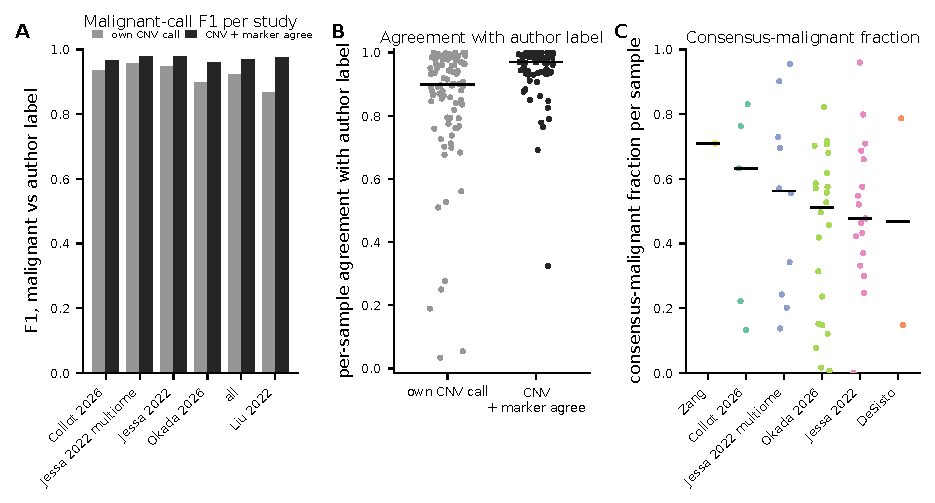
\includegraphics[width=0.95\textwidth]{figS1_malignant_calls.pdf}
\caption{\textbf{Malignant-cell calls.} \textbf{a}, F1 of the author-independent malignant calls against author labels
per study: own copy-number call, and cells where the copy-number and marker calls agree. \textbf{b}, Per-sample
agreement with author labels (samples with at least 100 compared cells). \textbf{c}, Fraction of consensus-malignant
cells per reference sample, by study.}\end{figure}

\begin{figure}[htbp]\centering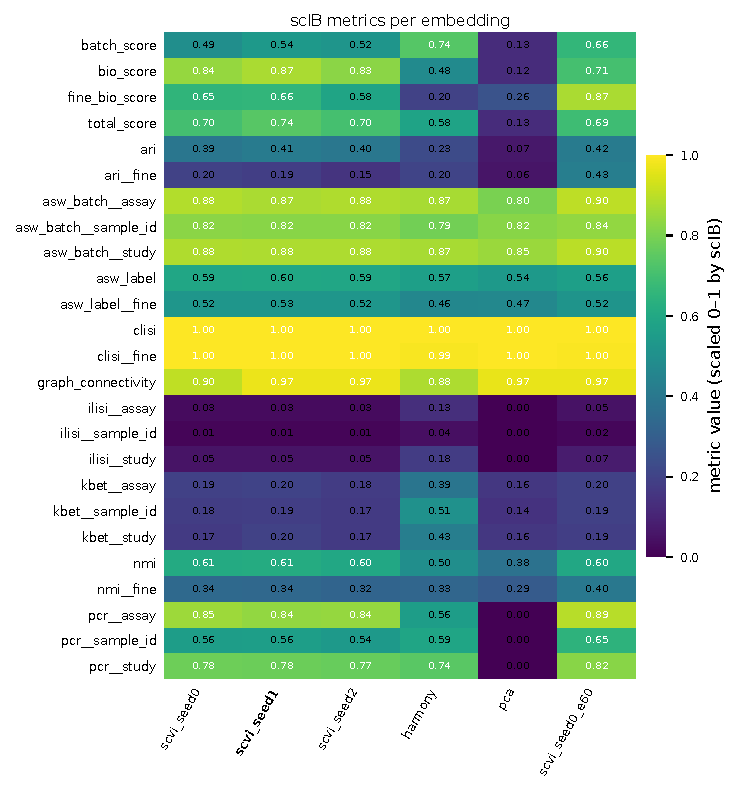
\includegraphics[width=0.95\textwidth]{figS2_integration_metrics.pdf}
\caption{\textbf{Integration benchmark.} All batch-correction metrics (batch keys sample, study, assay) and
biological-conservation metrics (coarse and fine labels) for the six candidate embeddings, with summary scores above.
Assay remains the hardest batch key for the chosen model.}\end{figure}

\begin{figure}[htbp]\centering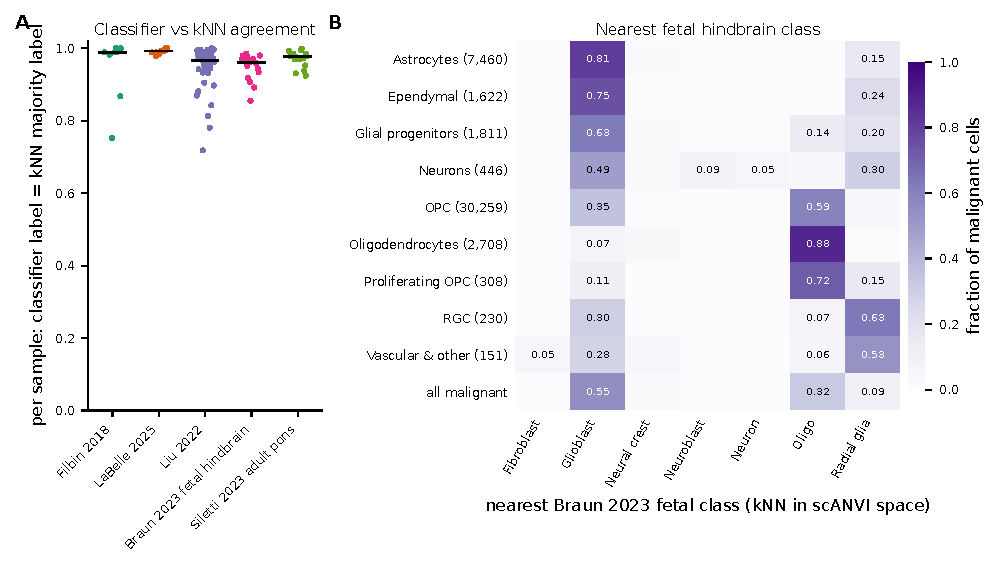
\includegraphics[width=0.95\textwidth]{figS3_mapping_origin.pdf}
\caption{\textbf{Mapping confidence and nearest fetal class.} \textbf{a}, Per-sample fraction of query cells whose
classifier label equals the majority label of their 15 nearest reference cells. \textbf{b}, Nearest fetal hindbrain
class of malignant cells, overall and by author state.}\end{figure}

\begin{figure}[htbp]\centering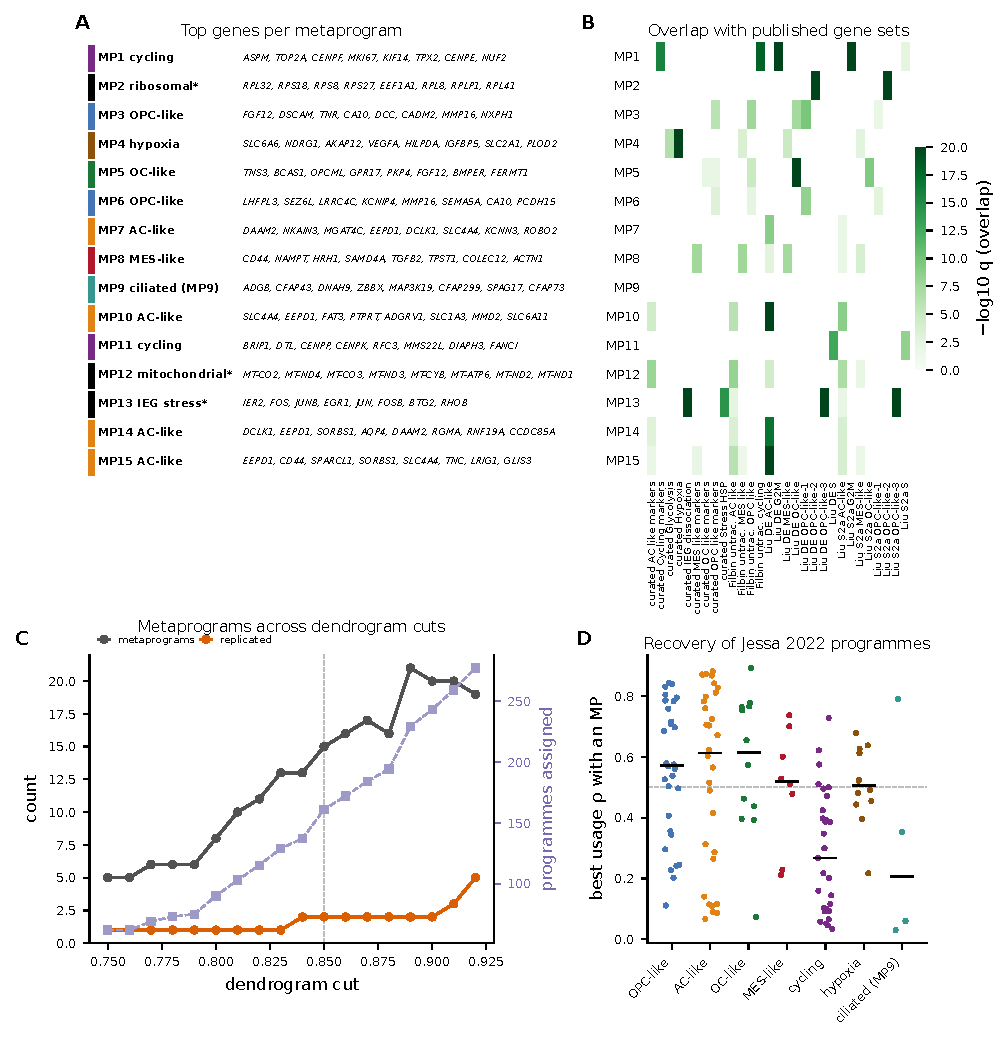
\includegraphics[width=0.95\textwidth]{figS4_metaprogram_detail.pdf}
\caption{\textbf{Metaprogram content and robustness.} \textbf{a}, Top eight genes of each metaprogram; a trailing
asterisk marks a technical programme. \textbf{b}, Overlap of metaprogram top-50 genes with published DMG and glioma
state gene sets (hypergeometric test, Benjamini--Hochberg $q$). \textbf{c}, Number of metaprograms, replicated
metaprograms and assigned programmes across dendrogram cuts. \textbf{d}, Best within-sample correlation of published
per-sample programmes with an atlas metaprogram.}\end{figure}

\begin{figure}[htbp]\centering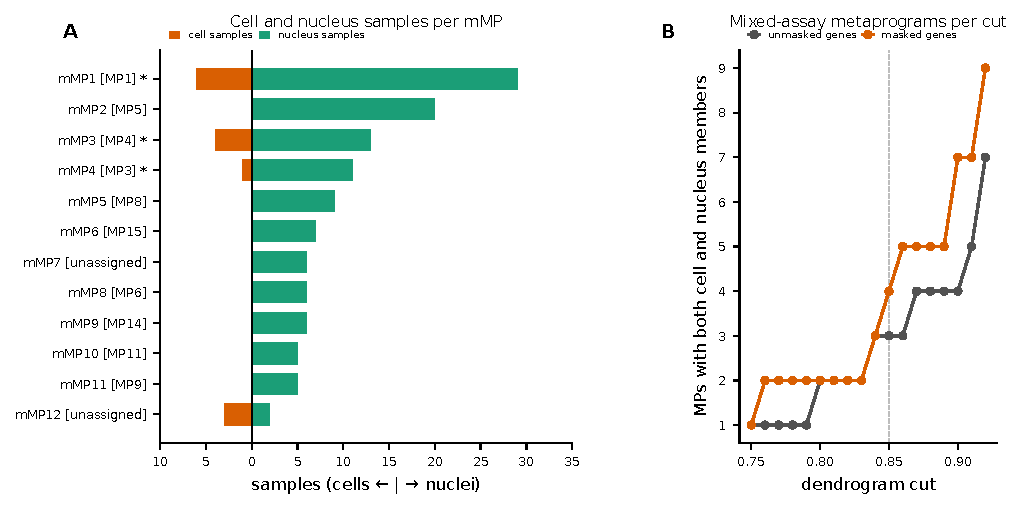
\includegraphics[width=0.95\textwidth]{figS5_masked_metaprograms.pdf}
\caption{\textbf{Metaprograms after masking assay-biased genes.} \textbf{a}, The 12 masked metaprograms at the primary
cut, with contributing cell and nucleus samples. \textbf{b}, Metaprograms containing both cell- and nucleus-derived
programmes across cuts, with all genes and after masking.}\end{figure}

\begin{figure}[htbp]\centering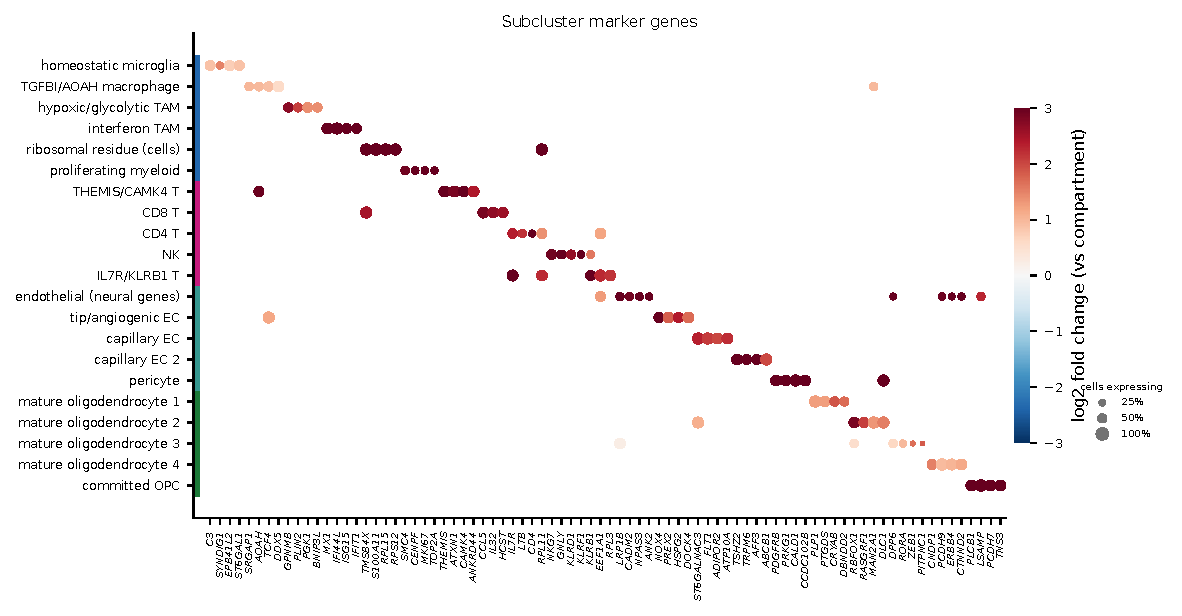
\includegraphics[width=0.95\textwidth]{figS6_tme_markers.pdf}
\caption{\textbf{Marker genes of the microenvironment subclusters.} Top four genes per subcluster; dot size is the
fraction of the subcluster's cells expressing the gene and colour the log fold change against the other subclusters of
the same compartment.}\end{figure}

\begin{figure}[htbp]\centering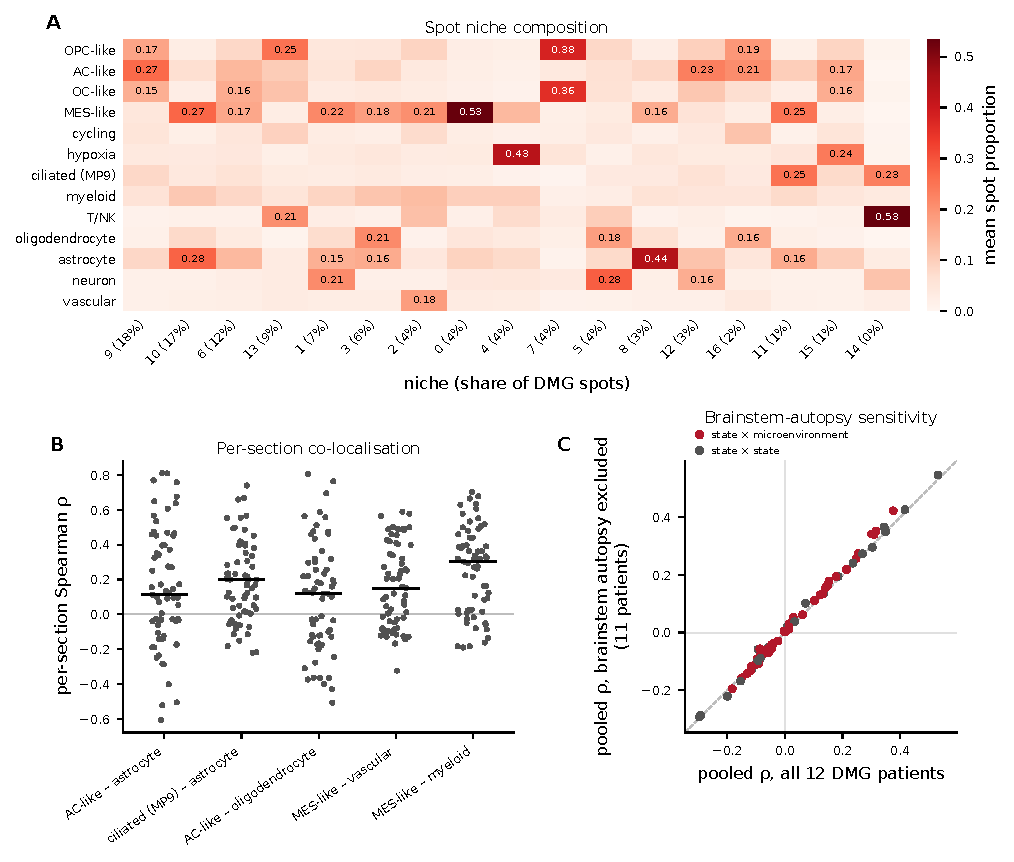
\includegraphics[width=0.95\textwidth]{figS7_spatial_detail.pdf}
\caption{\textbf{Spatial niches and sensitivity analyses.} \textbf{a}, Mean class proportions of the 16 spot niches.
\textbf{b}, Per-section correlations for the six strongest pairs of Figure~\ref{fig:spatial}d; every point is a
section, ten of which are serial sections of one autopsy. \textbf{c}, Pooled correlations with and without that
autopsy.}\end{figure}

\end{document}
